\chapter{MODELS}
%\chapter[short entry]{long title}
\label{chap:Proposed Methodology 1}
\section{Working Of ARIMA Model}
Weather forecasting is performed on Time Series Data. A time series is a sequence where a metric is recorded over regular time intervals. We use this type of series to forecast any event in the future such as temperature, rainfall, humidity, budgets etc.
\\
\\
For prediction we are going to use one of the most popular models for time series, Autoregressive Integrated Moving Average (ARIMA) which is a standard statistical model for time series forecast and analysis[8]. An ARIMA model can be understood by outlining each of its components as follows:
Autoregression (AR) - refers to a model that shows a changing variable that regresses on its own lagged, or prior, values. The notation AR (p) indicates an autoregressive model of order p.
\begin{equation}
      Yt = a + b1Yt-1 + b2Yt-2 + ...+bpYt-p + e1 
\end{equation}
● Integrated (I) - represents the differencing of raw observations to allow for the time series to become stationary, i.e., data values are replaced by the difference between the data values and the previous values
\textbf{Moving average (MA)} - incorporates the dependency between an observation and a residual error from a moving average model applied to lagged observations. The notation MA(q) refers to the moving average model of order q. 
\begin{equation}
   Y= a + et + et-1 + et-2+.... + qet-q
\end{equation}
Equation of the ARIMA model- Combination of AR and MA model 
\begin{equation}
   Yt = a + b1Yt-1 + b2Yt-2 + ...+bpYt-pet + et-1 + et-2+.... + qet-q 
\end{equation}
Before using the ARIMA model, we need to check whether the dataset is stationary or not. Check for below necessary conditions:
\\
 -->  Constant mean 
 \\
 -->  Constant variance 
 \\
 -->  An auto covariance that does not depend on time
\\
\\
If we have constant Mean and Variance, and our Test statistic is less than Critical Values, we already have a stationary Time series. So our 'd' value will become 0 in the ARIMA Model. And if it was non-stationary, in that case we would use below techniques to make it stationary by using any of the below techniques:
\\
 -->  Decomposing
 \\
 -->  Differencing
\\
\\
Auto ARIMA is a variance of ARIMA that is particularly useful for non-stationary datasets. Auto ARIMA saves the task of differencing and computing p, q, d values of ARIMA. Forecasting is done directly by fitting the Auto ARIMA model on the univariate time series data
\\
\\
\\
\\
\\
\\
\\
\section {Dataset Description}
 time series weather dataset is used to implement the ARIMA model of forecasting. The dataset contains weather data for Jhansi, India from year 2019 to 2023.This weather dataset includes several attributes such as temperature , humidity, atmospheric pressure etc. We apply the ARIMA model on various univariate time series from the Jhansi weather dataset.
 \\
 \\
 \\
Univariate time series is a time series that consists of only single observations recorded sequentially over equal time increments. Here, the ARIMA model of weather forecasting is applied to the temperature data from the weather dataset. The Auto ARIMA model of weather forecasting is applied to the temperature data from the weather dataset. Following are some data values from temperature and all the parameters in the  dataset respectively.
\\
\\
\\
 \begin{table}[htbp]
 \caption{Weather Dataset of Jhansi City}
     \begin{tabular}{@{}ccccccc@{}}
     \toprule
     Date & Temp-max & Temp-min 	& Atm-avg & Hum-max & Hum-min & Location\\
     \midrule
   2019-01-01 &26 & 6 & 1020 &	96 & 48 &	-Jhansi\\
   
2019-01-02	& 24 &	8 &	1020 &	94 & 58&	Jhansi\\

    2019-01-03& 25 & 8  & 1021 & 94  & 54 &	Jhansi\\
    
    2019-01-04 &23 & 8 & 1020 &	95 & 57& Jhansi\\
    
    2019-01-05 &24&	10&1018& 88& 54& Jhansi\\
    \bottomrule
     \end{tabular}
 \end{table}  
 \section {Materials and Methods}
The following process is used to implement the ARIMA model of weather forecasting on temperature data of Jhansi.
 \begin{description}
\item[Step-1:] Import statsmodels and pmdarima Python module for loading the ARIMA model. Import numpy, pandas, matplotlib, seaborn Python libraries for implementation and load the temperature dataset for ARIMA forecasting..
\begin{figure}[hbt!]
  \centering
  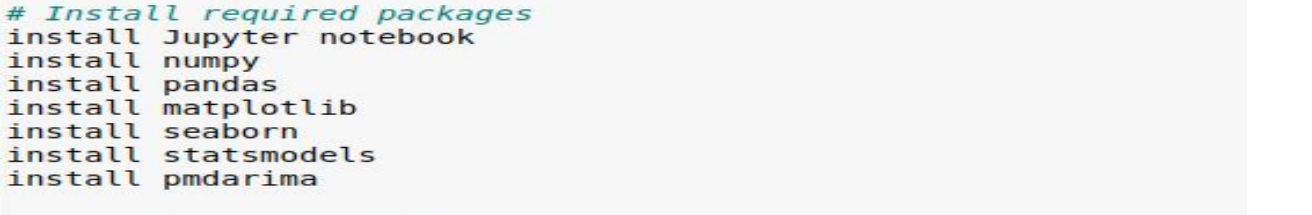
\includegraphics[width=0.8\linewidth]{images/outputs/1.png}
\end{figure}
\item[Step-2:] Import the required libraries
 \begin{figure}[hbt!]
  \centering
 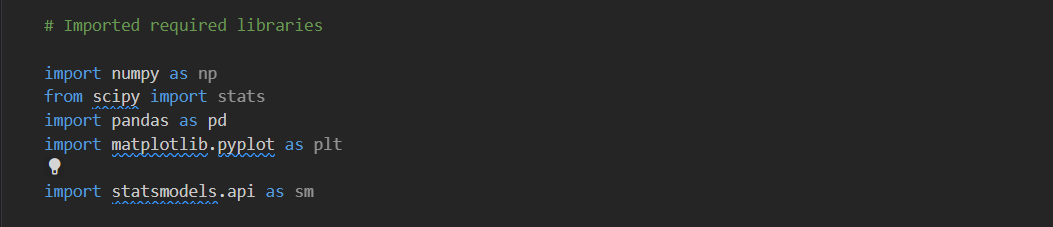
\includegraphics[width=0.8\linewidth]{images/outputs/2.png}
\end{figure}
\item[Step-3:] Load the data
 \begin{figure}[hbt!]
  \centering
  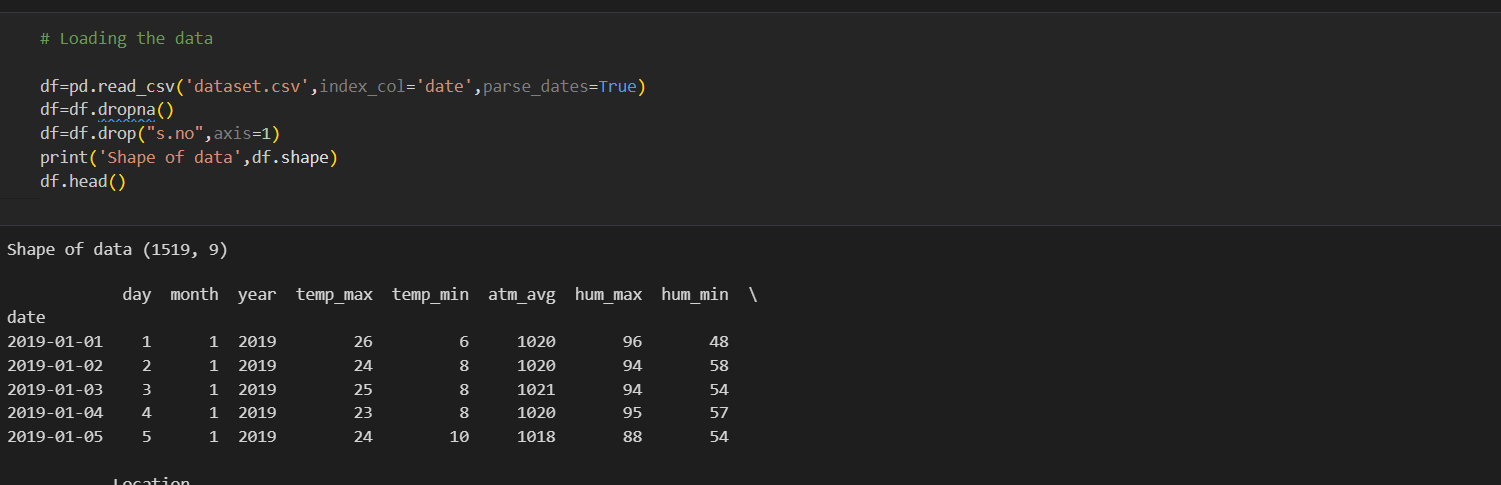
\includegraphics[width=0.8\linewidth]{images/outputs/3.png}
\end{figure}
\FloatBarrier
\pagebreak
\item[Step-4:] Plot the data to check the trend and seasonality of any parameter in the dataset

 \begin{figure}[hbt!]
  \centering
  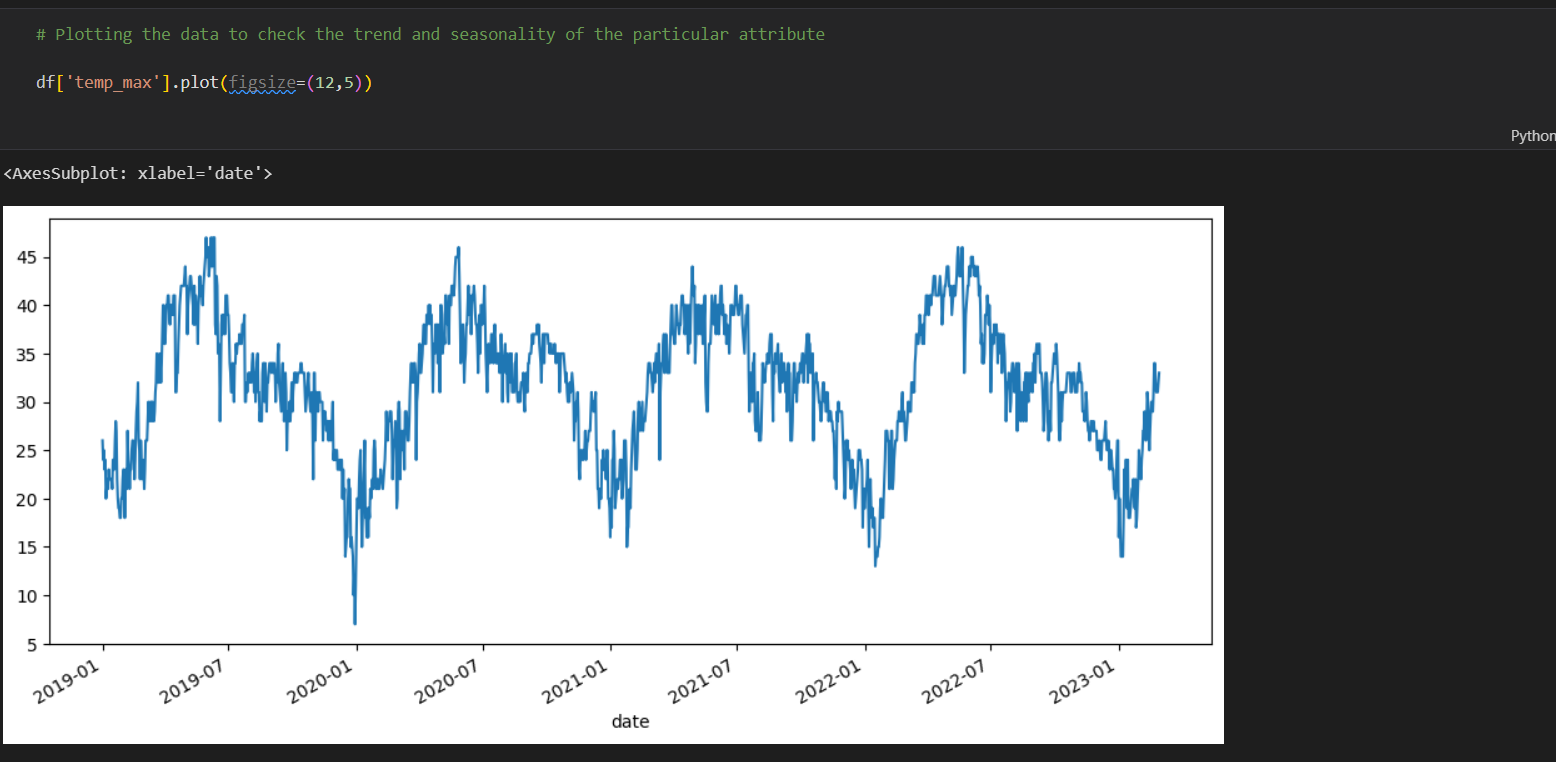
\includegraphics[width=0.7\linewidth]{images/outputs/4.png}
\end{figure}

\item[Step-5:] Perform the ad-fuller test to check the stationarity of the data

When we make a model for forecasting purposes in time series analysis,we require a stationary time series for better prediction.So the first step to work on modeling is to make a time series stationary.Testing for stationarity is a frequently used activity in autoregressive modeling.

ADF (Augmented Dickey-Fuller) test is a statistical significance test which means the test will give results in hypothesis tests with null and alternative hypotheses. As a result, we will have a p-value from which we will need to make inferences about the time series, whether it is stationary or not.

 \begin{figure}[hbt!]
  \centering
  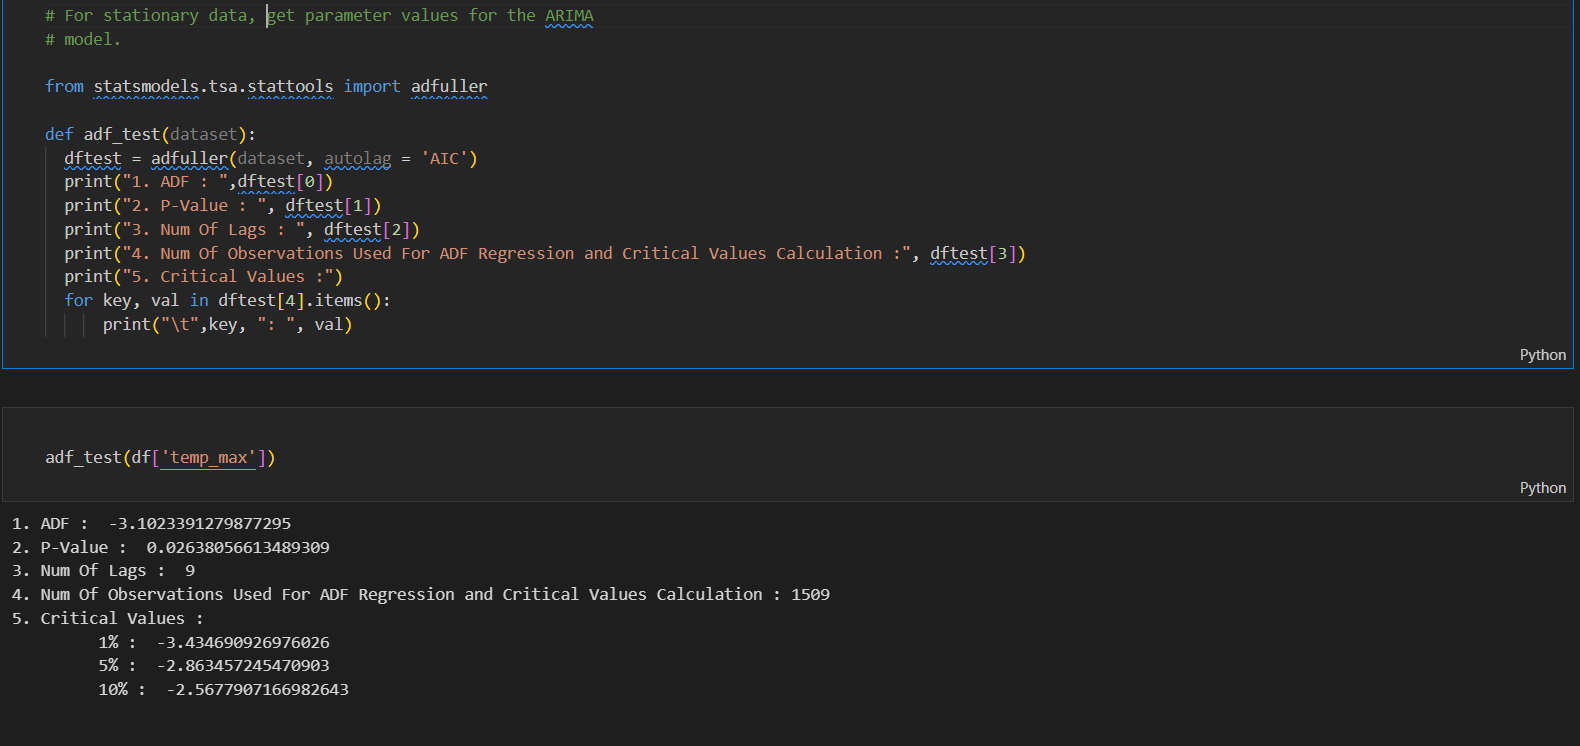
\includegraphics[width=0.8\linewidth]{images/outputs/5.png}
\end{figure}
Here in the results, we can see that the p-value for time series is greater than 0.05, and we can say we fail to reject the null hypothesis and the time series is non-stationary.
\pagebreak
\item[Step-6:] For forecasting non-stationary data, the Auto ARIMA model is used

 \begin{figure}[hbt!]
  \centering
  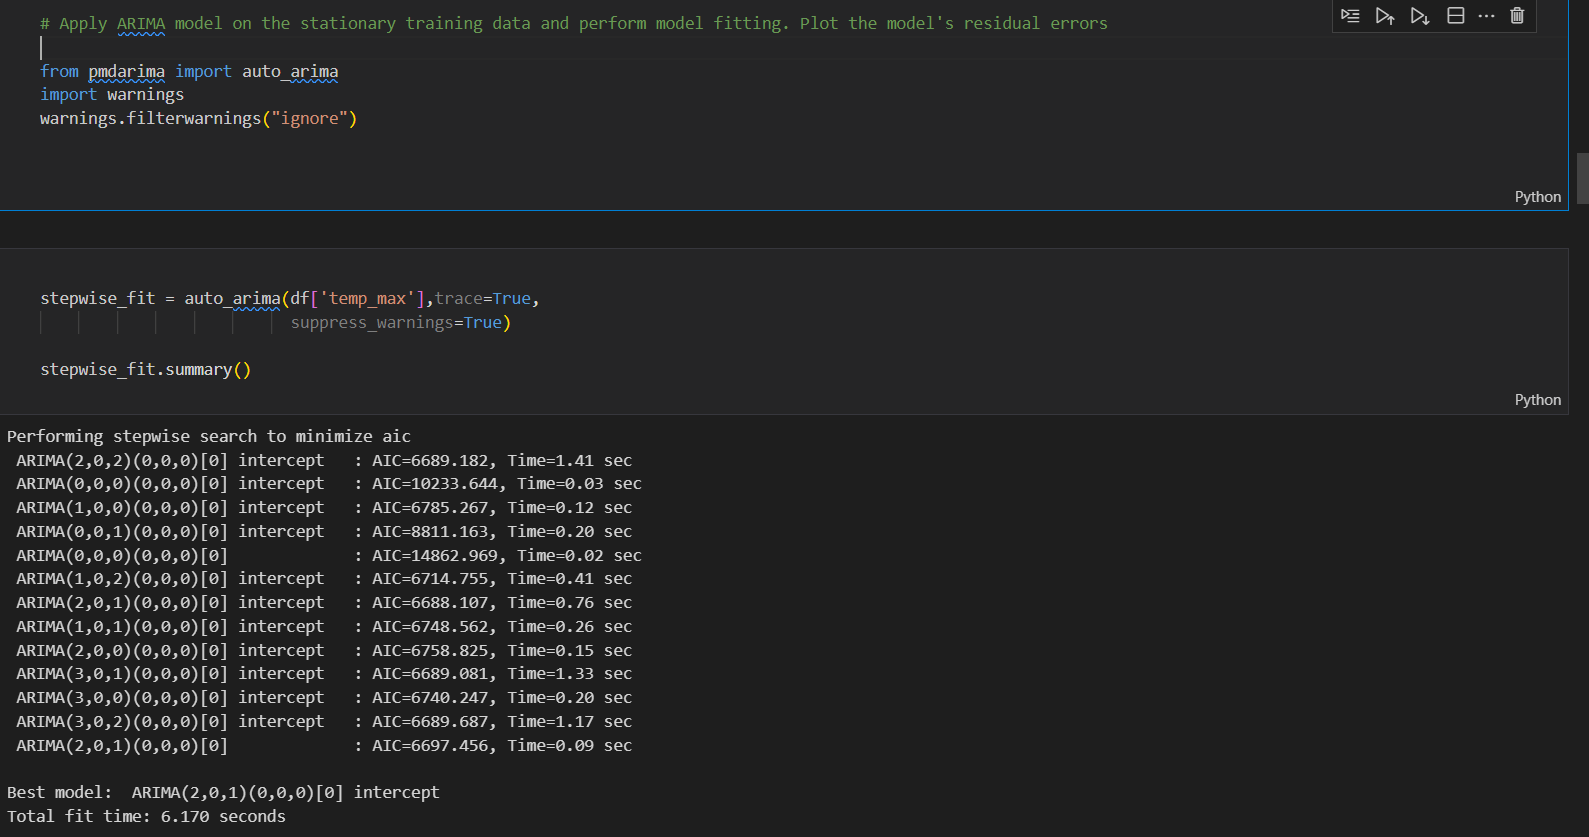
\includegraphics[width=0.8\linewidth]{images/outputs/6.png}
\end{figure}

The best model which came out to be used is(2,0,1) the
 A non seasonal ARIMA model is classified as an "ARIMA(p,d,q)" model, where:
 
 p is the number of autoregressive terms,

d is the number of nonseasonal differences needed for stationarity, and

q is the number of lagged forecast errors in the prediction equation.

\textbf{Summary of the model}

 \begin{figure}[hbt!]
  \centering
  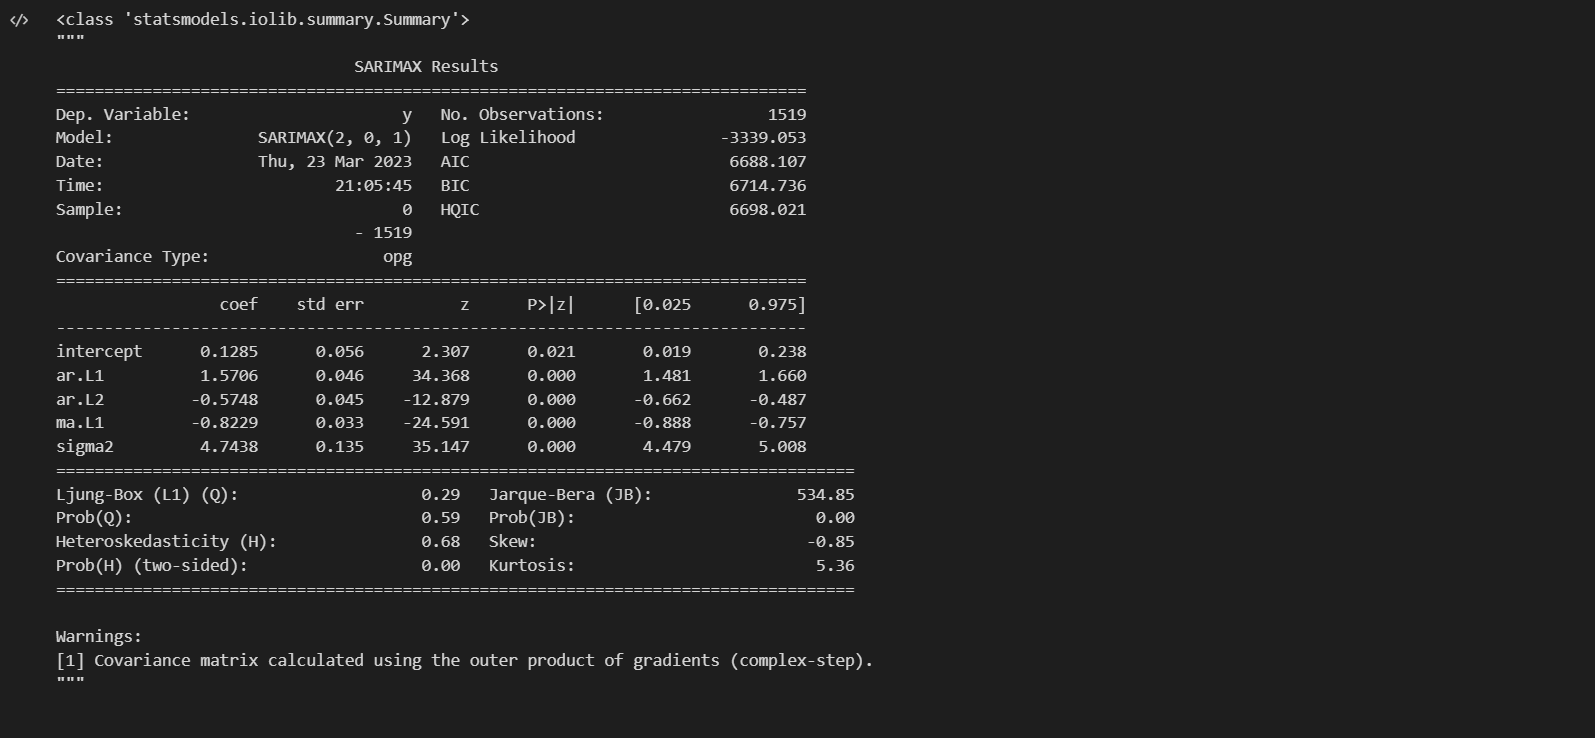
\includegraphics[width=0.8\linewidth]{images/outputs/7.png}
\end{figure}

\pagebreak
\item[Step-7:] Set the testing and training part

 \begin{figure}[hbt!]
  \centering
  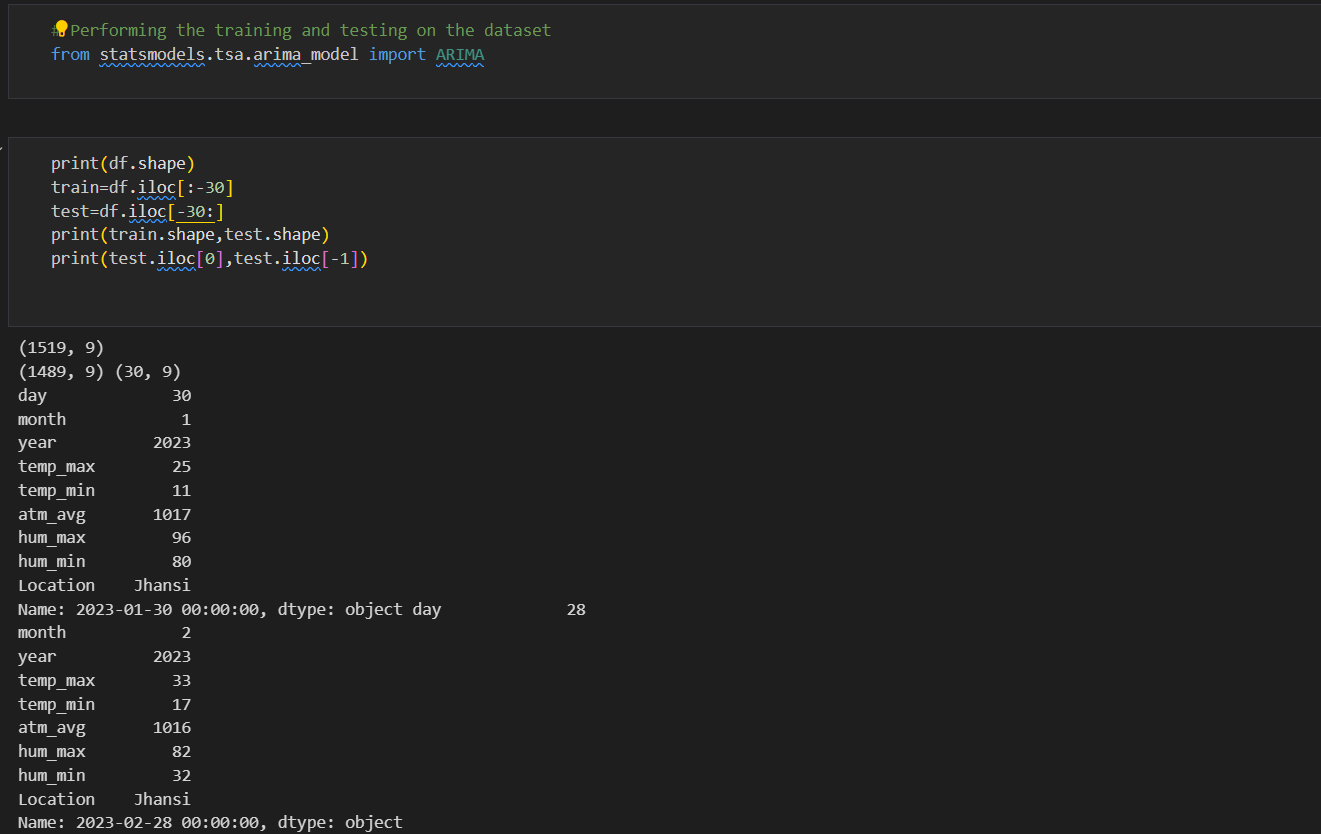
\includegraphics[width=0.7\linewidth]{images/outputs/8.png}
\end{figure}

\item[Step-8:] Testing our model on the remaining datasets and plotting to see the difference, what was the temperature according to dataset and what the model has predicted
 \begin{figure}[hbt!]
  \centering
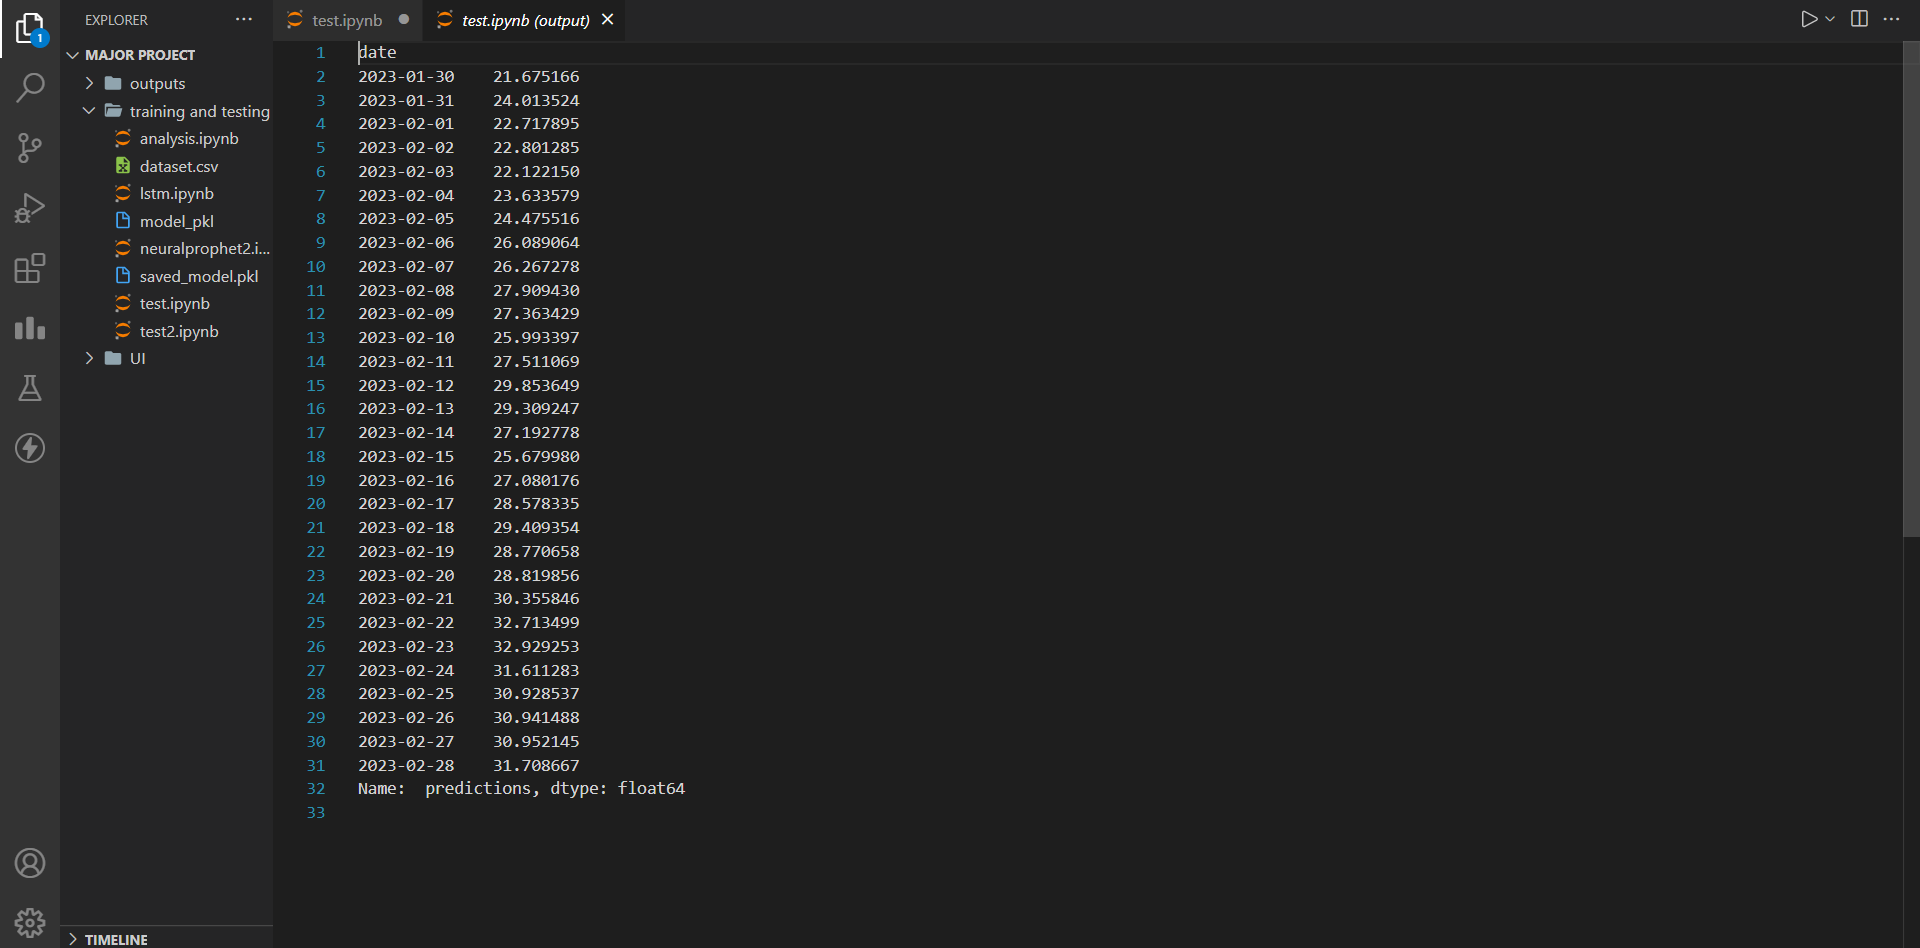
\includegraphics[width=0.7\linewidth]{images/outputs/9.png}
\end{figure}

\begin{figure}[hbt!]
  \centering 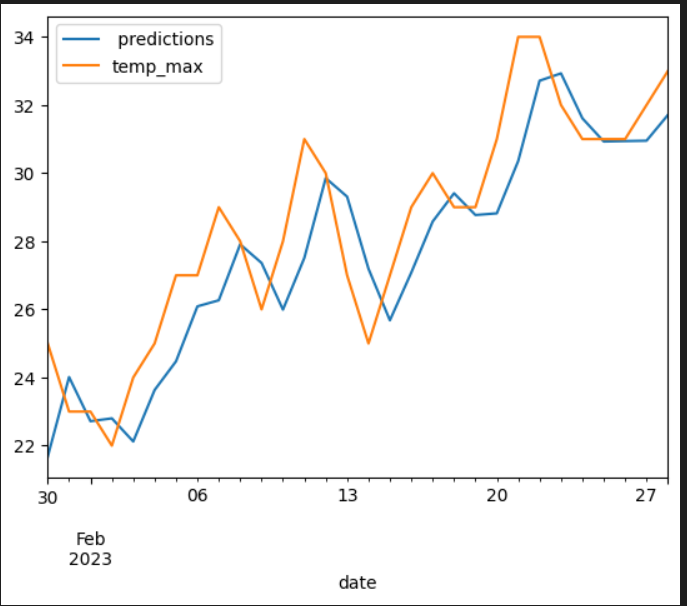
\includegraphics[width=0.5\linewidth]{images/outputs/11.png}
  \caption{Training and Testing Output}
\end{figure}

\item[Step-9:] Now the most important part comes where we have to predict that particular parameter for the future dates as per the requirements

 \begin{figure}[hbt!]
  \centering
  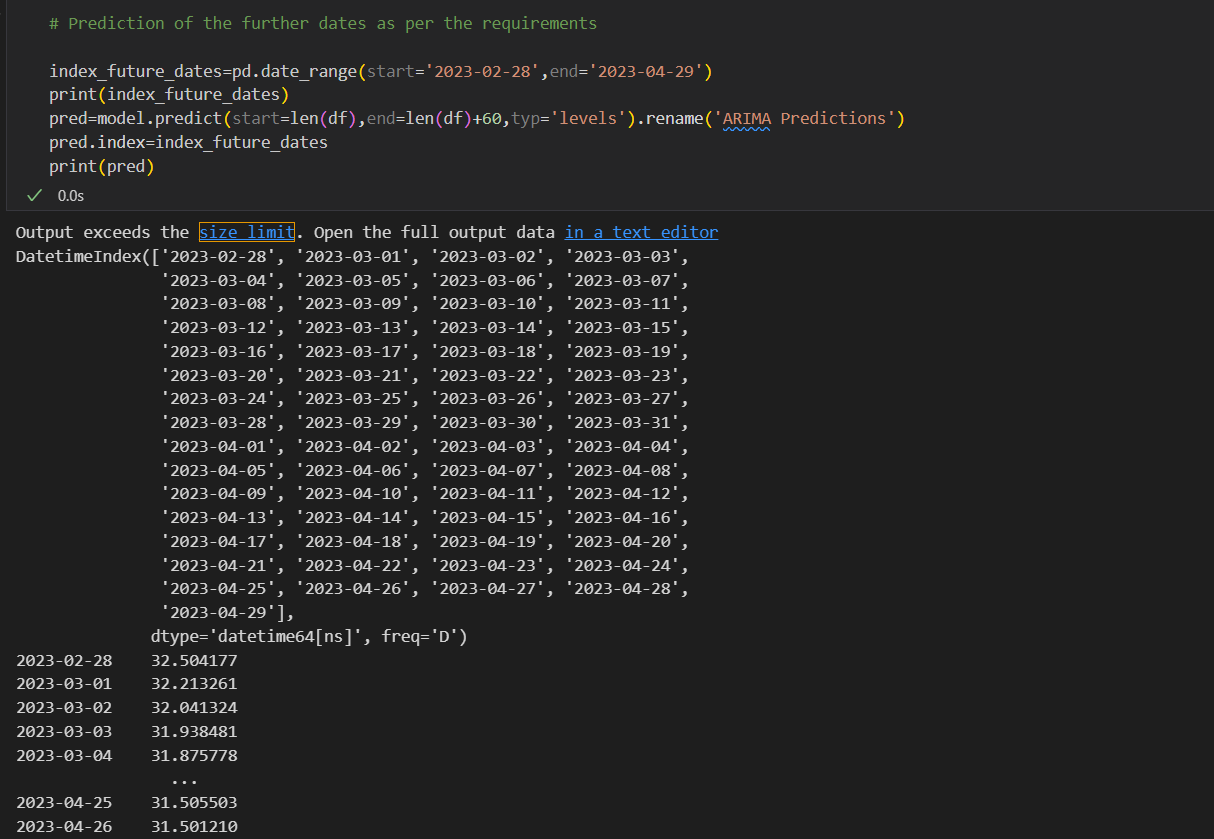
\includegraphics[width=0.8\linewidth]{images/outputs/12.png}
\end{figure}
 

\item[Step-10:] Plot of the graph and the table of the values are as follows:
 \begin{figure}[hbt!]
  \centering
  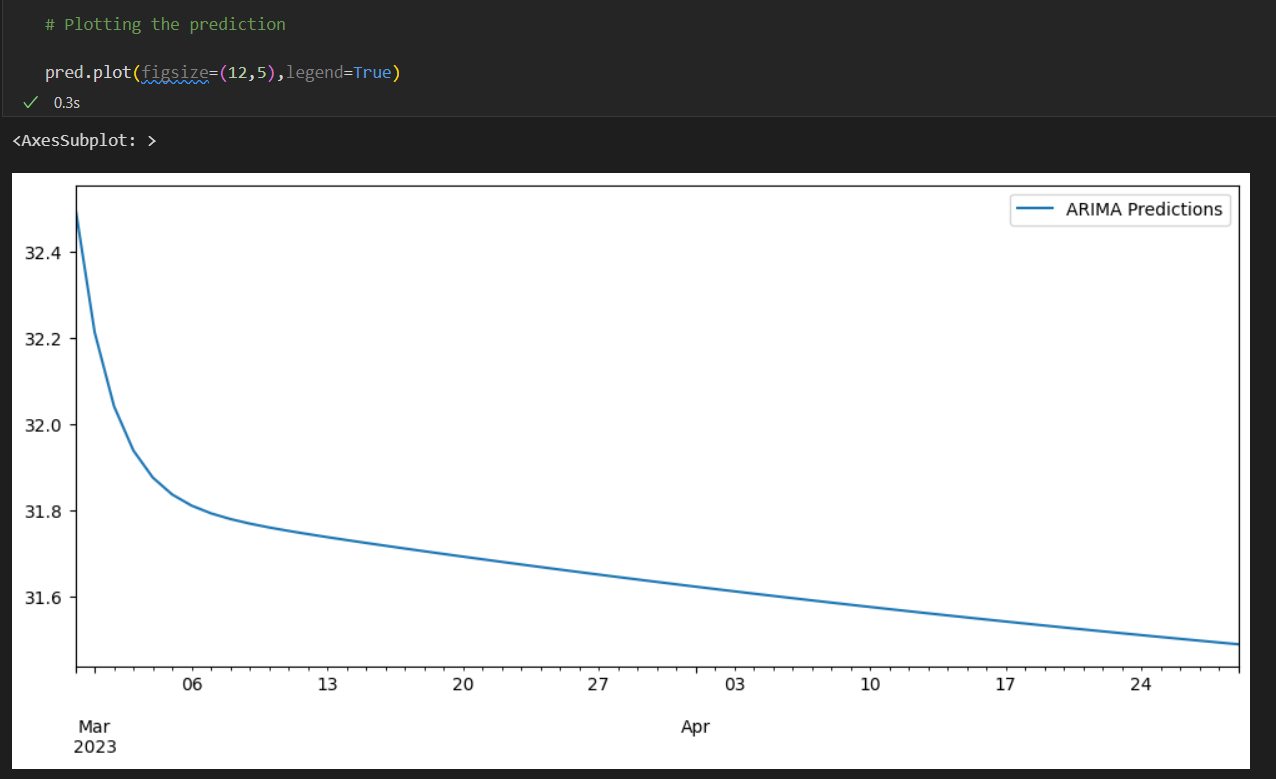
\includegraphics[width=0.8\linewidth]{images/outputs/13.png}
\end{figure}
 
\end{description}
\pagebreak
\section{Weather Forecasting using Neural Network}
Artificial neural networks (ANNs) have emerged as a result of the discovery of the computer, the advancement of technology, the ability to store data regularly, and the ability of computers to think, problem-solve, remember and learn[10]. We are presenting weather predictions using Artificial Neural Network and Back Propagation Algorithm. We are implementing a data intensive model using data mining techniques. Weather is a dynamic and non-linear process and an artificial neural network (ANN) can deal with such a Process. 
We are using ANN which is based on smart analyzing the trend from historical data. The other models are accurate in calculation but not in predictions as they are not able to adapt the irregular patterns of data which can neither be written in the form of function or deducted as formula[11].
Use of ANN will give more accurate results. Here, the error may or may not reduce completely. But, the accuracy will improve as compared to previous forecasts.
\begin{figure}[hbt!]
  \centering
  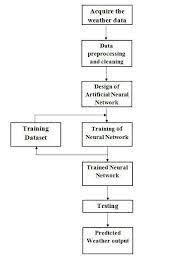
\includegraphics[width=0.5 \linewidth]{images/outputs/imageeee.jpeg}
  \caption{Flow chart Of Neural Network Model Working}
\end{figure}
 

\section{ Procedure to develop model}
To develop an ANN model for weather forecasting, region selection for input data and parameters is necessary. The input data is to be taken from a specific area on which the model is trained and tested so that the model is able to generate accurate results[12]. The number of input data given to the model also helps to improve accuracy of the model by giving the results with a high degree of similarity between predicted and actual output data. The available data may be noisy , data should be cleaned. 

Similarly, it has to be normalized because all the parameters are of different units and normalization will help the input and output parameters to correlate with each other . The data should be divided in training and testing samples in proper proportion so that the results can be predicted, tested and validated properly. Structure of the NN model also has a great impact on the generation of accurate results[13].

As the weather data is nonlinear, Artificial Neural Network (ANN) has become an effective way of predicting weather data precisely and accurately[14]. Neural Network is a system that can be trained with certain input and output. It creates its own structure based upon how it is trained.

\pagebreak
\section{Back-Propagation Approach}
The back propagation algorithm is used in layered feedforward ANNs. It uses supervised learning, which means the model trains itself with the use of target output. For every set of input data the target output is provided. The neural network model processes the input data with random values for weights and suitable activation function using one or more hidden layers in between and then produces the predicted output[15]. This predicted output is then compared with the target output provided for the same input dataset. Thus, error is calculated by subtracting predicted output from target output. Using this error, the weights are adjusted and again the entire process is repeated for multiple epochs until the error is minimal or in acceptable range[16] . 


We start the training with random weights, and the goal is to adjust them so that the error will be minimal. The area for input data can be any one of a meteorological station area in which all the data is limited to a certain region. The different input parameters are taken viz. temperature, relative humidity, rainfall,etc.Input data is then pre-processed and cleaned. That means it is checked with any outlier and that is missing values are entered, and data is checked if it is in the given range for the given parameter.


 Later ANN is designed with a number of input and output nodes, hidden layers, activation function, and maximum number of epochs, weights, bias, goal and learning function. Neural network is trained with seventy percent of the input data. Where the model is trained using this observed data to forecast the weather. Then the mean squared error and accuracy is calculated for the model by comparing the output of testing with target output. This model generates output in terms of minimum and maximum temperature of the day, relative humidity[17].
The back propagation (BP) neural network algorithm is a multi-layer feedforward network trained according to error back propagation algorithm and is one of the most widely applied neural network models. BP network can be used to learn and store a great deal of mapping relations of input-output model, and no need to disclose in advance the mathematical equation that describes these mapping relations. Its learning rule is to adopt the steepest descent method in which the back propagation is used to regulate the weight value and threshold value of the network to achieve the minimum error sum of square[18].
 \pagebreak
 \section{Methods}
 The following process is used to implement the Neural Network model of weather forecasting on temperature data of Jhansi.
 \begin{description} 


\item[Step-1:] Import the required libraries.


 \begin{figure}[hbt!]
  \centering
  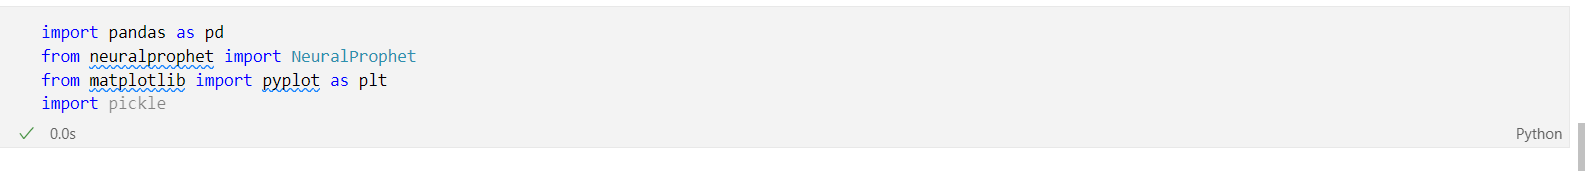
\includegraphics[width=0.8\linewidth]{images/outputs/import.png}
\end{figure}



\item[Step-2:] Read the dataset


 \begin{figure}[hbt!]
  \centering
  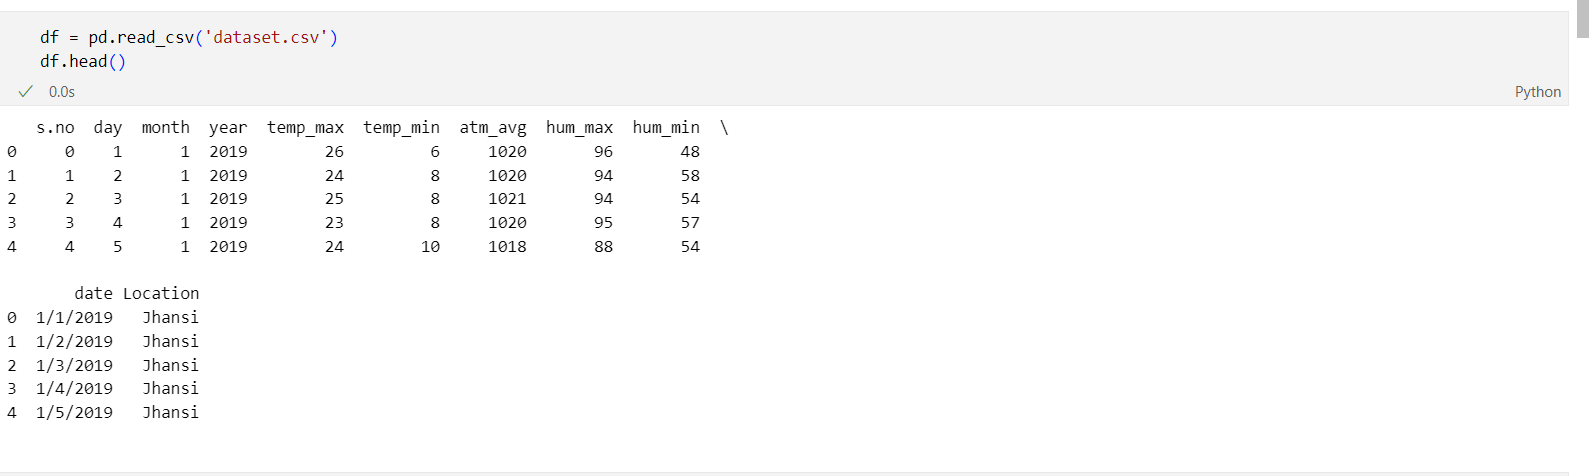
\includegraphics[width=0.8\linewidth]{images/outputs/dataset reading.png}
\end{figure}


\item[Step-3:] Setting the location as unique as there would be no problems if any other city is present in the dataset

 \begin{figure}[hbt!]
  \centering
  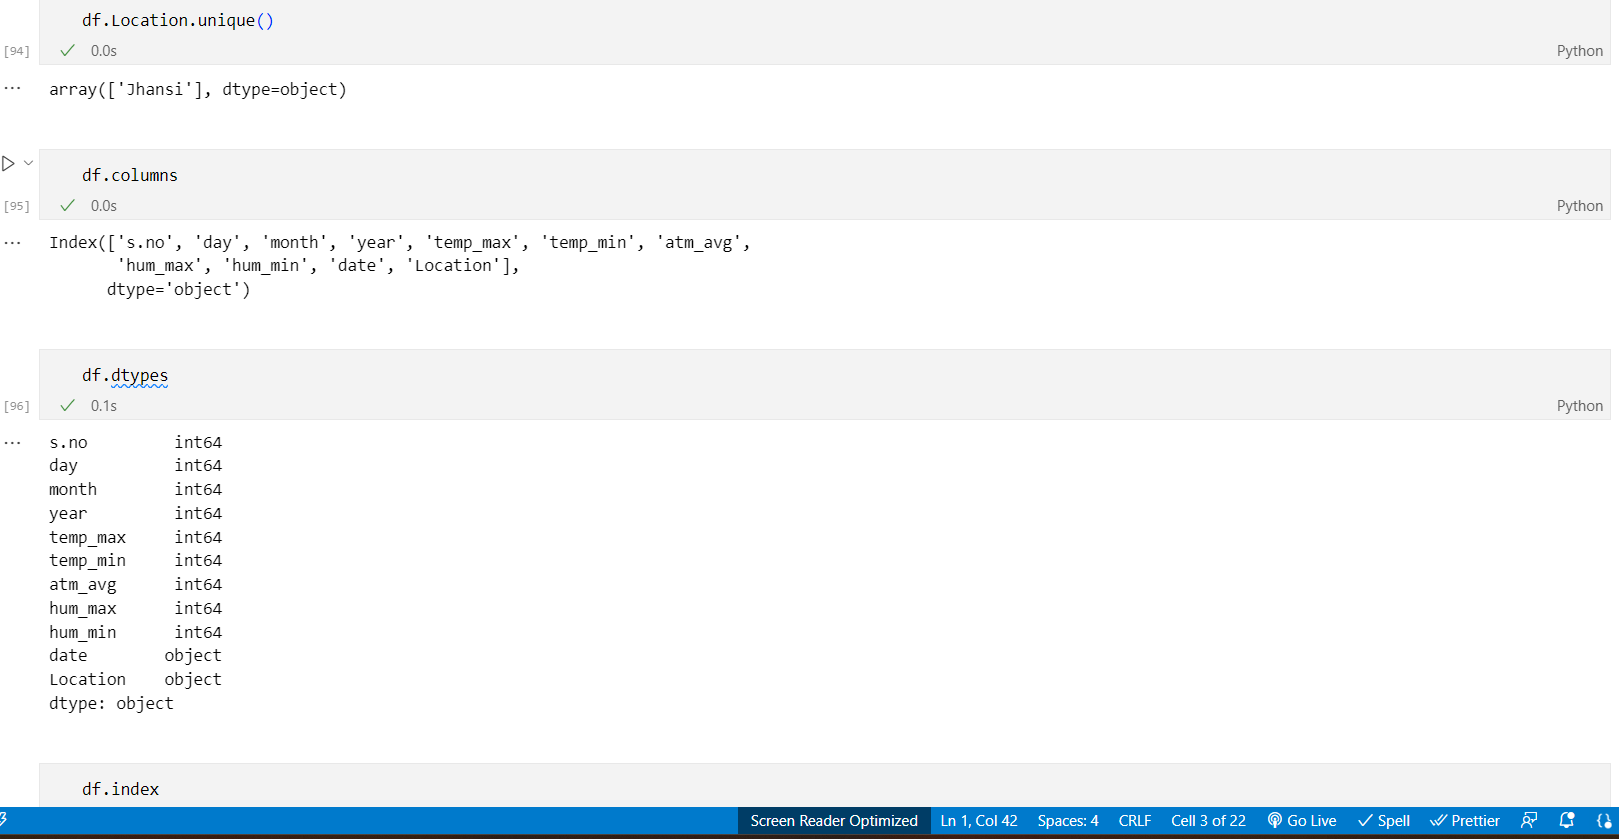
\includegraphics[width=0.8\linewidth]{images/outputs/unique.png}
\end{figure}


\pagebreak
\item[Step-4:] Importing and fitting and training the model

 \begin{figure}[hbt!]
  \centering
  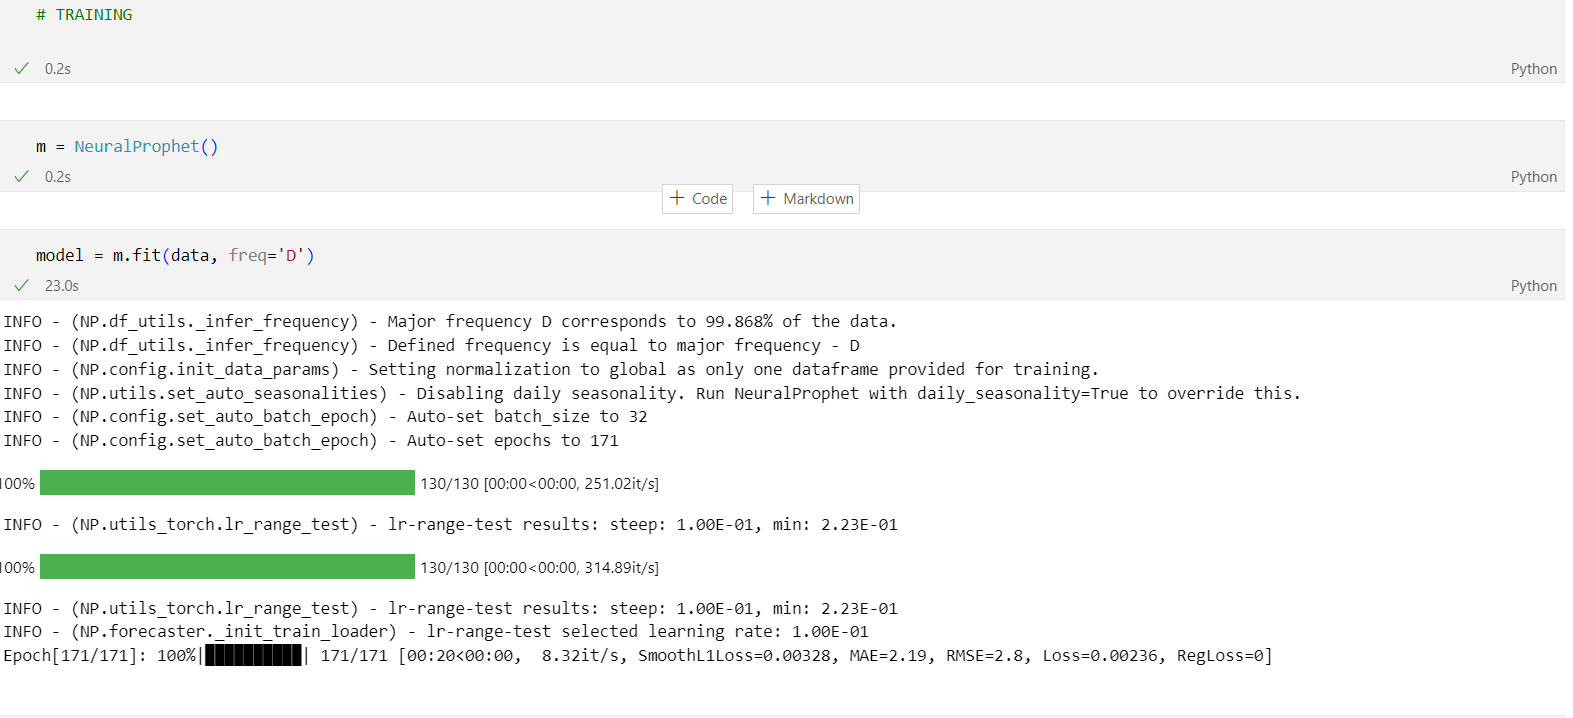
\includegraphics[width=0.7\linewidth]{images/outputs/model.png}
\end{figure}


\item[Step-5:] .Making the Future predictions and plotting it

 \begin{figure}[hbt!]
  \centering
  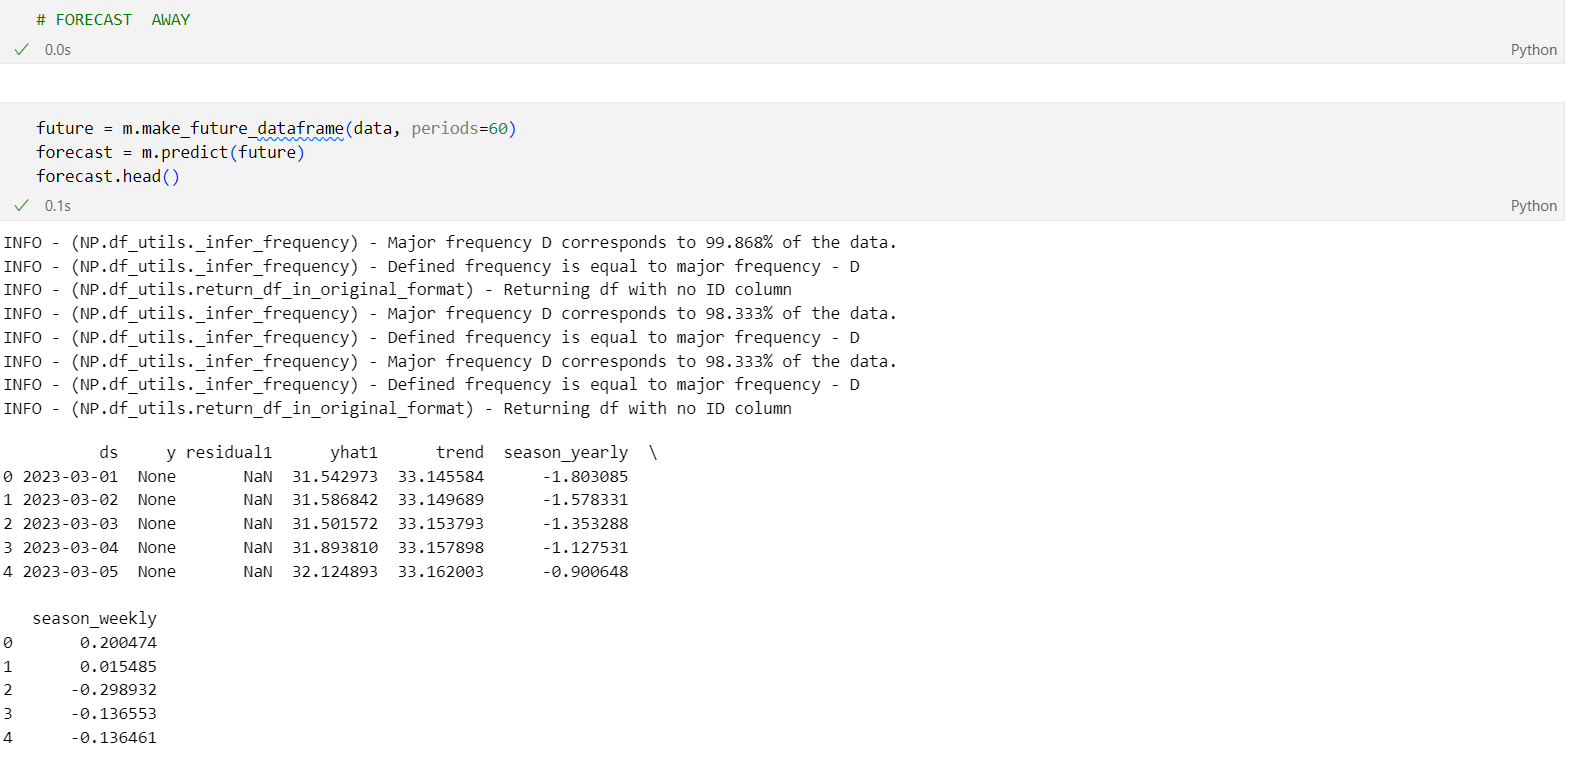
\includegraphics[width=0.8\linewidth]{images/outputs/forecast.png}
\end{figure}

\item[Step-6:] Forecast Plotting

 \begin{figure}[hbt!]
  \centering
  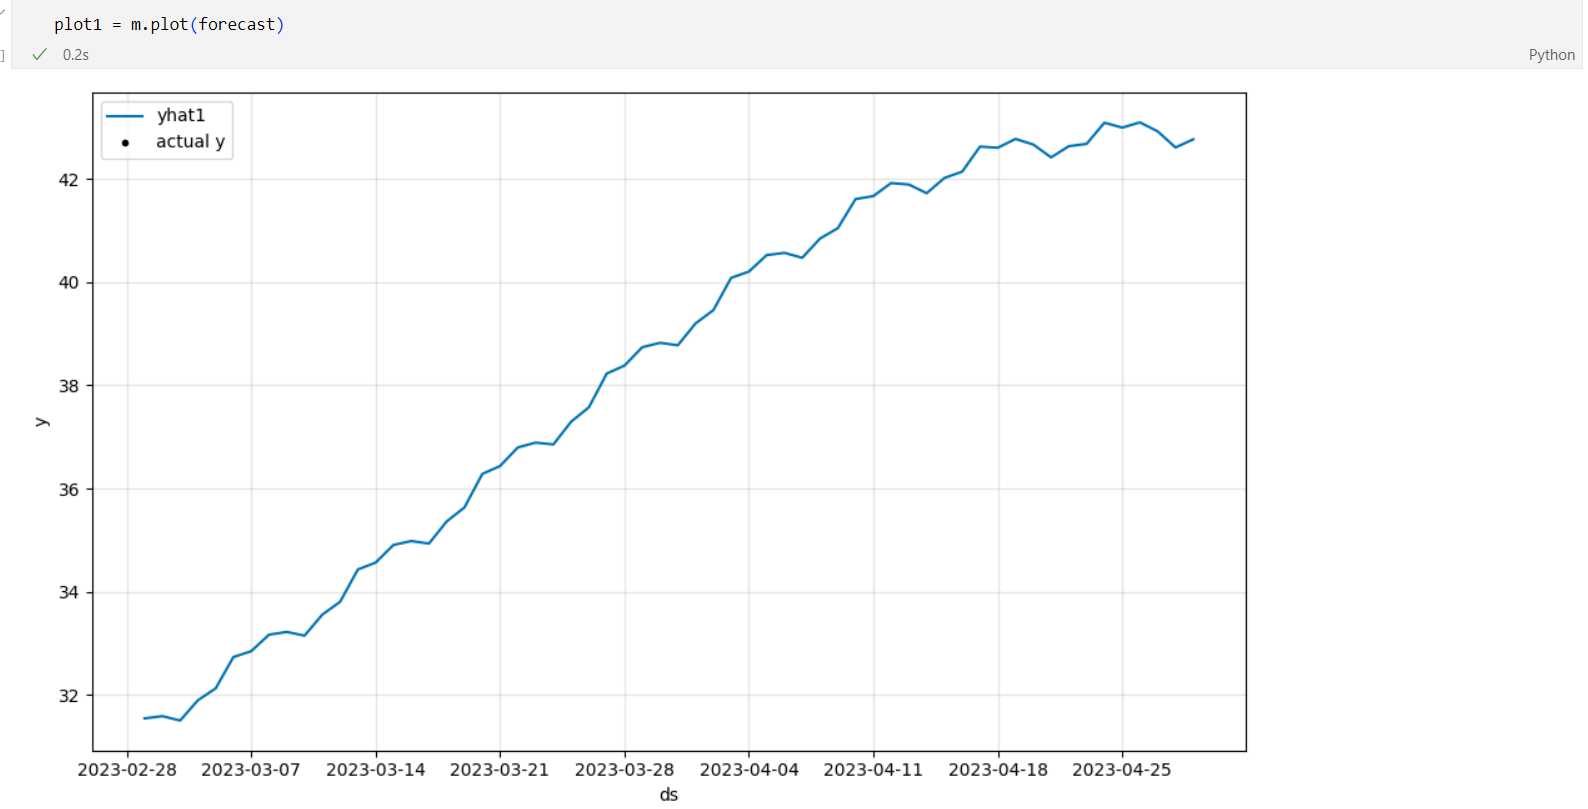
\includegraphics[width=0.8\linewidth]{images/outputs/plot.png}
  \caption{Forecast Of Maximum Temperature for time span of 2 Months of NN Mode}
\end{figure}

\pagebreak
\item[Step-7:] Component Plotting

\begin{figure}[hbt!]
  \centering
  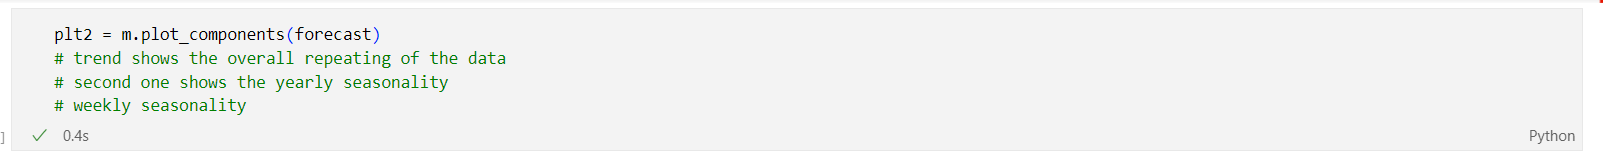
\includegraphics[width=0.7\linewidth]{images/outputs/component plotting.png}
\end{figure}


 \begin{figure}[hbt!]
  \centering
  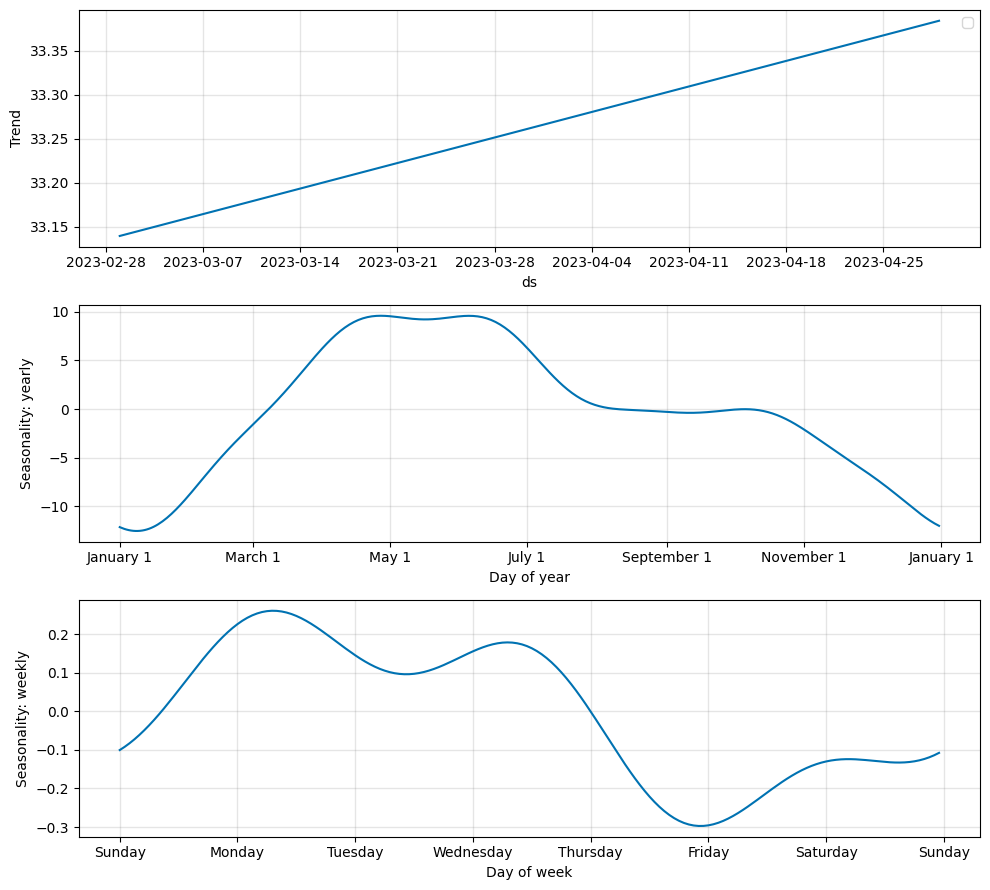
\includegraphics[width=0.7\linewidth]{images/outputs/neural temp_max trend.png}
  \caption{Components Plotting of Maximum Temperature}
\end{figure}

\end{description}
\pagebreak
\section{Predictions  of various parameters through neural networks:}
\textbf{1. Minimum Temperature}
\begin{figure}[hbt!]
  \centering
  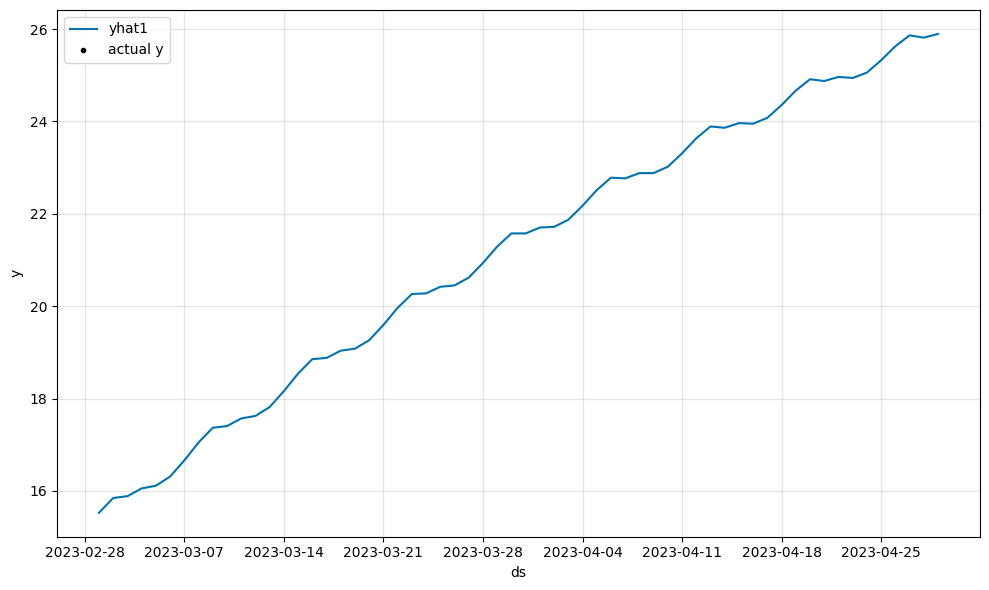
\includegraphics[width=0.7\linewidth]{images/outputs/neural temp_min.png}
  \caption{Plot of Minimum Temperature by NN Model}
\end{figure}


 \begin{figure}[hbt!]
  \centering
  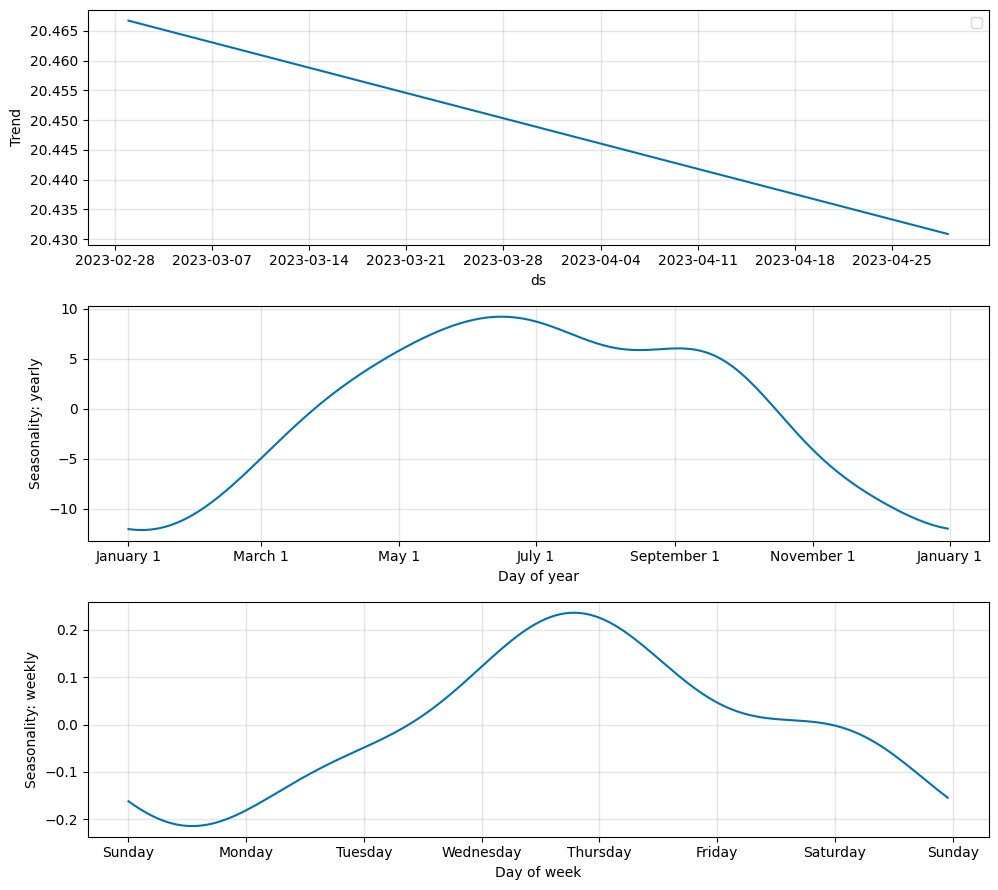
\includegraphics[width=0.7\linewidth]{images/outputs/neural temp_min trend.png}
  \caption{Components Plotting of Minimum Temperature}
\end{figure}



\textbf{2. Minimum Humidity}
\begin{figure}[hbt!]
  \centering
  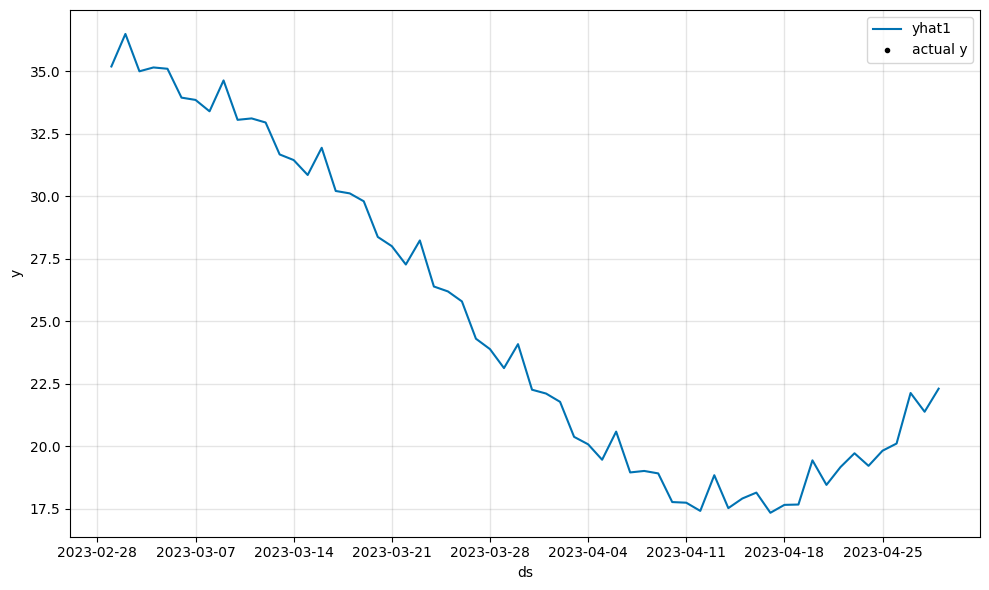
\includegraphics[width=0.7\linewidth]{images/outputs/neural hum_min.png}
  \caption{Plot of Minimum Humidity by NN Model}
\end{figure}


 \begin{figure}[hbt!]
  \centering
  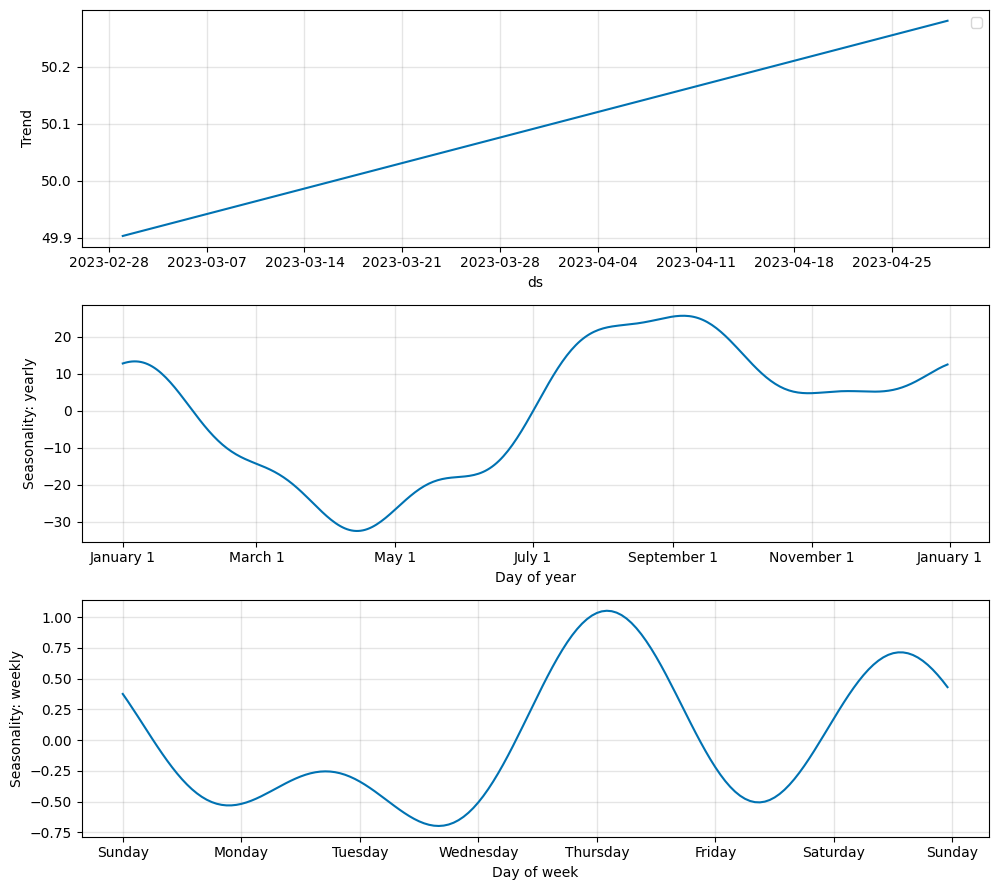
\includegraphics[width=0.7\linewidth]{images/outputs/neural hum_min trend.png}
  \caption{Components Plotting of Minimum Humidity}
\end{figure}

\textbf{3. Maximum Humidity}
\begin{figure}[hbt!]
  \centering
  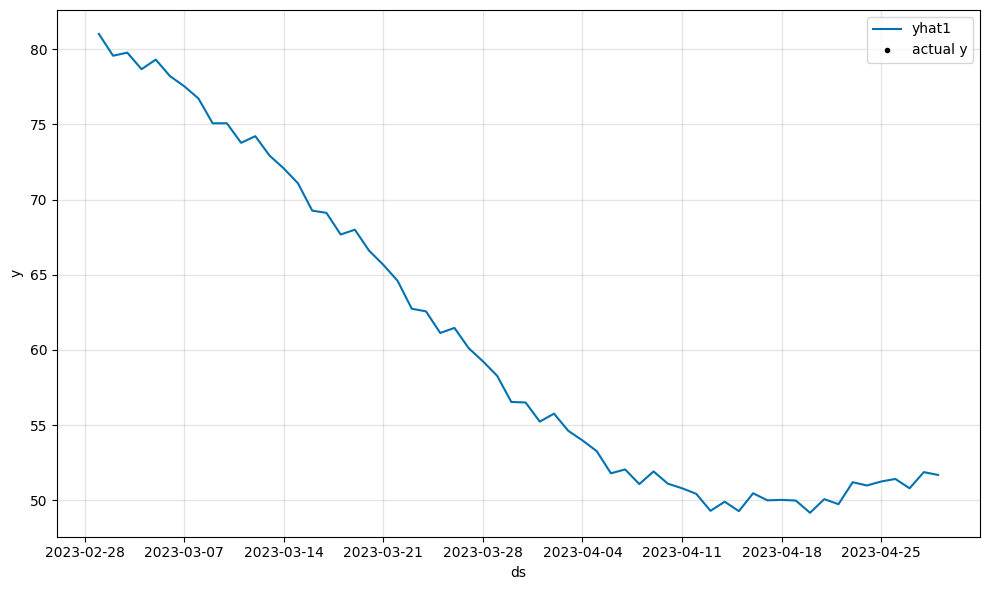
\includegraphics[width=0.7\linewidth]{images/outputs/neural hum_max.png}
  \caption{Plot of Maximum Humidity by NN Model}
\end{figure}


 \begin{figure}[hbt!]
  \centering
  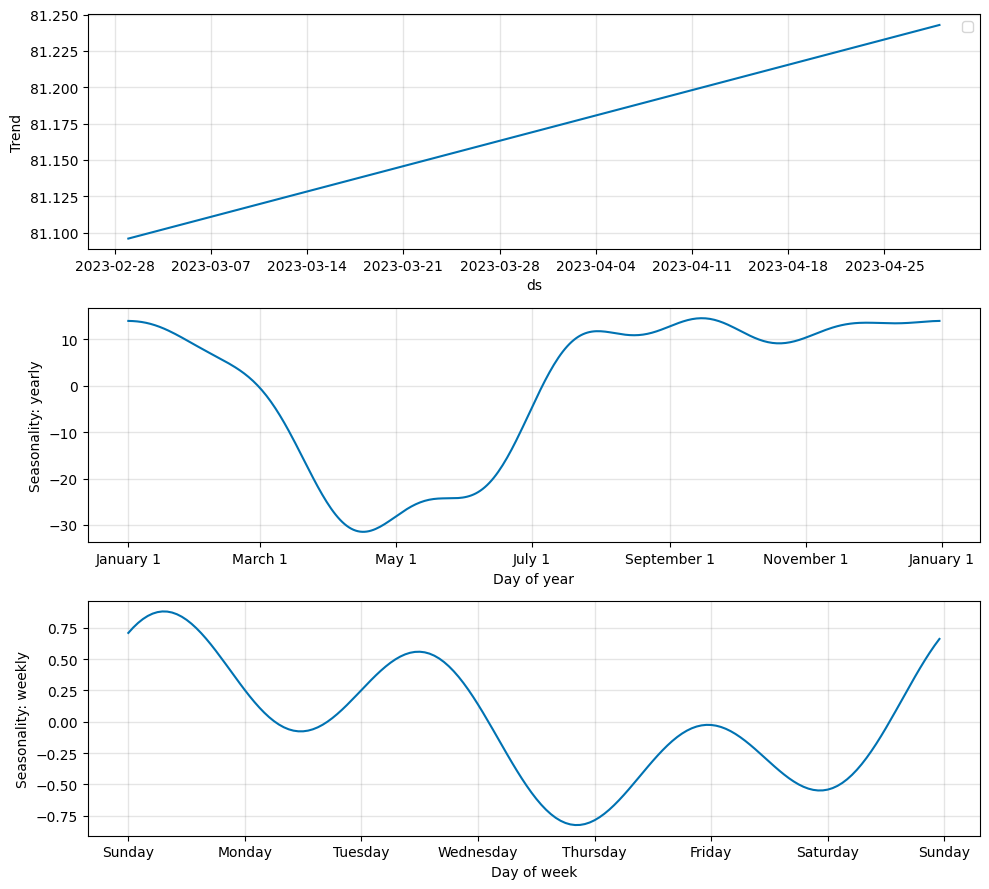
\includegraphics[width=0.7\linewidth]{images/outputs/neural hum_max trend.png}
  \caption{Components Plotting of Maximum Humidity}
\end{figure}
